\documentclass[tikz,border=10pt]{standalone}
\usetikzlibrary{calc}
\usetikzlibrary{decorations.pathmorphing}

\makeatletter

% gluon decoration (based on the original coil decoration)

\pgfdeclaredecoration{gluon}{coil}
{
  \state{coil}[switch if less than=%
    0.5\pgfdecorationsegmentlength+%>
    \pgfdecorationsegmentaspect\pgfdecorationsegmentamplitude+%
    \pgfdecorationsegmentaspect\pgfdecorationsegmentamplitude to last,
               width=+\pgfdecorationsegmentlength]
  {
    \pgfpathcurveto
    {\pgfpoint@oncoil{0    }{ 0.555}{1}}
    {\pgfpoint@oncoil{0.445}{ 1    }{2}}
    {\pgfpoint@oncoil{1    }{ 1    }{3}}
    \pgfpathcurveto
    {\pgfpoint@oncoil{1.555}{ 1    }{4}}
    {\pgfpoint@oncoil{2    }{ 0.555}{5}}
    {\pgfpoint@oncoil{2    }{ 0    }{6}}
    \pgfpathcurveto
    {\pgfpoint@oncoil{2    }{-0.555}{7}}
    {\pgfpoint@oncoil{1.555}{-1    }{8}}
    {\pgfpoint@oncoil{1    }{-1    }{9}}
    \pgfpathcurveto
    {\pgfpoint@oncoil{0.445}{-1    }{10}}
    {\pgfpoint@oncoil{0    }{-0.555}{11}}
    {\pgfpoint@oncoil{0    }{ 0    }{12}}
  }
  \state{last}[next state=final]
  {
    \pgfpathcurveto
    {\pgfpoint@oncoil{0    }{ 0.555}{1}}
    {\pgfpoint@oncoil{0.445}{ 1    }{2}}
    {\pgfpoint@oncoil{1    }{ 1    }{3}}
    \pgfpathcurveto
    {\pgfpoint@oncoil{1.555}{ 1    }{4}}
    {\pgfpoint@oncoil{2    }{ 0.555}{5}}
    {\pgfpoint@oncoil{2    }{ 0    }{6}}
  }
  \state{final}{}
}

\def\pgfpoint@oncoil#1#2#3{%
  \pgf@x=#1\pgfdecorationsegmentamplitude%
  \pgf@x=\pgfdecorationsegmentaspect\pgf@x%
  \pgf@y=#2\pgfdecorationsegmentamplitude%
  \pgf@xa=0.083333333333\pgfdecorationsegmentlength%
  \advance\pgf@x by#3\pgf@xa%
}

\makeatother
\begin{document}
  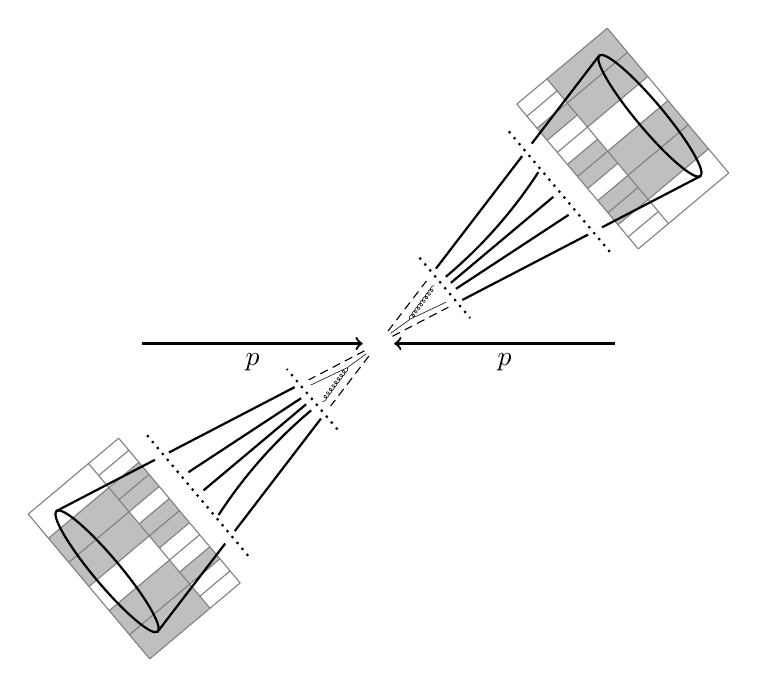
\begin{tikzpicture}
    % \draw [<->,thick] (-6,0) -- (6,0) node (yaxis) [above] {$z$};
    % \draw [<->,thick] (0,-4) -- (0,4) node (yaxis) [above] {$y$};
    \draw[thick, ->] (-3,0) -- (-0.2,0) node[below, midway] {$p$};
    \draw[thick, ->] (3,0) -- (0.2,0) node[below, midway] {$p$};
      \begin{scope}[rotate=-50]
        % Detector
        \fill[fill=lightgray] (-0.8,3.3) rectangle (-0.6,3.8);
        \fill[fill=lightgray] (-0.2,3.3) rectangle (-0.0,3.8);
        \fill[fill=lightgray] (-0.0,3.3) rectangle (0.2,3.8);
        \fill[fill=lightgray] (0.4,3.3) rectangle (0.6,3.8);
        \fill[fill=lightgray] (0.4,3.3) rectangle (0.8,3.8);

        \fill[fill=lightgray] (0.4,3.8) rectangle (0.8,4.8);
        \fill[fill=lightgray] (0.0,3.8) rectangle (0.4,4.8);
        \fill[fill=lightgray] (-1.2,3.8) rectangle (-0.8,4.8);
        \fill[fill=lightgray] (-0.8,3.8) rectangle (-0.4,4.8);

        \draw[gray] (-1.2,3.3) -- (-1.2,4.8);
        \draw[gray] (1.2,3.3) -- (1.2,4.8);
        \draw[gray] (1.0,3.3) -- (1.0,3.8);
        \draw[gray] (0.8,3.3) -- (0.8,3.8);
        \draw[gray] (0.6,3.3) -- (0.6,3.8);
        \draw[gray] (0.4,3.3) -- (0.4,3.8);
        \draw[gray] (0.2,3.3) -- (0.2,3.8);
        \draw[gray] (0.0,3.3) -- (0.0,3.8);
        \draw[gray] (-1.0,3.3) -- (-1.0,3.8);
        \draw[gray] (-0.8,3.3) -- (-0.8,3.8);
        \draw[gray] (-0.6,3.3) -- (-0.6,3.8);
        \draw[gray] (-0.4,3.3) -- (-0.4,3.8);
        \draw[gray] (-0.2,3.3) -- (-0.2,3.8);

        \draw[gray] (-0.0,3.8) -- (-0.0,4.8);
        \draw[gray] (-0.4,3.8) -- (-0.4,4.8);
        \draw[gray] (-0.8,3.8) -- (-0.8,4.8);
        \draw[gray] (0.4,3.8) -- (0.4,4.8);
        \draw[gray] (0.8,3.8) -- (0.8,4.8);

        \draw[gray] (-1.2,3.3) -- (1.2,3.3);
        \draw[gray] (-1.2,4.8) -- (1.2,4.8);
        \draw[gray] (-1.2,3.8) -- (1.2,3.8);

        % end of detector

      % \clip (-2,0) rectangle (2,-1cm);
        \coordinate (A) at (0,0);
        \coordinate (B) at (-1,4.5);
        \coordinate (C) at (1,4.5);
        \draw[thick] (0,4.5) circle(1cm and 0.17cm);
        \draw[densely dashed] ($(A)!0.2cm!(B)$) -- ($(A)!1.0cm!(B)$);
        \draw[densely dashed] ($(A)!0.2cm!(C)$) -- ($(A)!1.0cm!(C)$);
        \draw[thick] ($(A)!1.2cm!(B)$) -- ($(A)!3.0cm!(B)$);
        \draw[thick] ($(A)!1.2cm!(C)$) -- ($(A)!3.0cm!(C)$);
        \draw[thick] ($(A)!3.2cm!(B)$) -- (B);
        \draw[thick] ($(A)!3.2cm!(C)$) -- (C);

        \draw[thick,dotted] (-0.5,1.1) -- (0.5, 1.1);
        \draw[thick,dotted] (-1.0,3.0) -- (1.0, 3.0);

        % parton level
        \path (0.02,0.5) edge[very thin, decorate,decoration={gluon, amplitude=0.7pt, segment length=1.6pt, aspect=1.1}] (-0.1,1.0);
        \draw[very thin] (0.0,0.2) -- (0.02, 0.5);
        \draw[very thin] (0.02,0.5) -- (0.15, 1.0);
        % particle level
        \draw[thick] (0.1,1.2) -- (0.3, 2.9);
        \draw[thick] (0.0,1.2) -- (0.0, 2.9);
        % \draw[thick, bend left=40] (-0.1,1.2) -- (-0.3, 2.9);
        \draw[thick] (-0.1,1.2) arc (0:17:6cm);

      \end{scope}
      \begin{scope}[rotate=-230]
        % Detector
        \fill[fill=lightgray] (-0.8,3.3) rectangle (-0.6,3.8);
        \fill[fill=lightgray] (-0.2,3.3) rectangle (-0.0,3.8);
        \fill[fill=lightgray] (-0.0,3.3) rectangle (0.2,3.8);
        \fill[fill=lightgray] (0.4,3.3) rectangle (0.6,3.8);
        \fill[fill=lightgray] (0.4,3.3) rectangle (0.8,3.8);

        \fill[fill=lightgray] (0.4,3.8) rectangle (0.8,4.8);
        \fill[fill=lightgray] (0.0,3.8) rectangle (0.4,4.8);
        \fill[fill=lightgray] (-1.2,3.8) rectangle (-0.8,4.8);
        \fill[fill=lightgray] (-0.8,3.8) rectangle (-0.4,4.8);

        \draw[gray] (-1.2,3.3) -- (-1.2,4.8);
        \draw[gray] (1.2,3.3) -- (1.2,4.8);
        \draw[gray] (1.0,3.3) -- (1.0,3.8);
        \draw[gray] (0.8,3.3) -- (0.8,3.8);
        \draw[gray] (0.6,3.3) -- (0.6,3.8);
        \draw[gray] (0.4,3.3) -- (0.4,3.8);
        \draw[gray] (0.2,3.3) -- (0.2,3.8);
        \draw[gray] (0.0,3.3) -- (0.0,3.8);
        \draw[gray] (-1.0,3.3) -- (-1.0,3.8);
        \draw[gray] (-0.8,3.3) -- (-0.8,3.8);
        \draw[gray] (-0.6,3.3) -- (-0.6,3.8);
        \draw[gray] (-0.4,3.3) -- (-0.4,3.8);
        \draw[gray] (-0.2,3.3) -- (-0.2,3.8);

        \draw[gray] (-0.0,3.8) -- (-0.0,4.8);
        \draw[gray] (-0.4,3.8) -- (-0.4,4.8);
        \draw[gray] (-0.8,3.8) -- (-0.8,4.8);
        \draw[gray] (0.4,3.8) -- (0.4,4.8);
        \draw[gray] (0.8,3.8) -- (0.8,4.8);

        \draw[gray] (-1.2,3.3) -- (1.2,3.3);
        \draw[gray] (-1.2,4.8) -- (1.2,4.8);
        \draw[gray] (-1.2,3.8) -- (1.2,3.8);

        % end of detector

      % \clip (-2,0) rectangle (2,-1cm);
        \coordinate (A) at (0,0);
        \coordinate (B) at (-1,4.5);
        \coordinate (C) at (1,4.5);
        \draw[thick] (0,4.5) circle(1cm and 0.17cm);
        \draw[densely dashed] ($(A)!0.2cm!(B)$) -- ($(A)!1.0cm!(B)$);
        \draw[densely dashed] ($(A)!0.2cm!(C)$) -- ($(A)!1.0cm!(C)$);
        \draw[thick] ($(A)!1.2cm!(B)$) -- ($(A)!3.0cm!(B)$);
        \draw[thick] ($(A)!1.2cm!(C)$) -- ($(A)!3.0cm!(C)$);
        \draw[thick] ($(A)!3.2cm!(B)$) -- (B);
        \draw[thick] ($(A)!3.2cm!(C)$) -- (C);

        \draw[thick,dotted] (-0.5,1.1) -- (0.5, 1.1);
        \draw[thick,dotted] (-1.0,3.0) -- (1.0, 3.0);

        % parton level
        \path (0.02,0.5) edge[very thin, decorate,decoration={gluon, amplitude=0.7pt, segment length=1.6pt, aspect=1.1}] (-0.1,1.0);
        \draw[very thin] (0.0,0.2) -- (0.02, 0.5);
        \draw[very thin] (0.02,0.5) -- (0.15, 1.0);
        % particle level
        \draw[thick] (0.1,1.2) -- (0.3, 2.9);
        \draw[thick] (0.0,1.2) -- (0.0, 2.9);
        % \draw[thick, bend left=40] (-0.1,1.2) -- (-0.3, 2.9);
        \draw[thick] (-0.1,1.2) arc (0:17:6cm);

      \end{scope}


    % \draw[thick,->] (0,-4) -- node[left,font=\footnotesize] {$x$} (0,1);
    % \draw (aa) -| (bb);
  \end{tikzpicture}
\end{document}
